\chapter{Parametric Benchmarks} \label{chp:parametric}
\section{Introduction} \label{sec:parametric/introduction}
As we have already investigated in section \ref{sec:runtime/analysis}, there are multiple kinds of dependency and hazards. In order to complete a thorough analysis, a new kind of benchmark has been developed in order to analyse the effect of the three kinds of dependency.

\section{Problem Statement} \label{sec:parametric/problem}
The problem statement is somewhat simple. Given $n$ accesses, generate patterns of access such that there are $n^{\delta}$, $n^{\delta^{0}}$ and $n^{\delta^{-1}}$ dependencies. These values are by definition probabilistic in nature, as the issue of array aliasing is important.

In this context, we consider an \textit{access pattern} to be two sequential accesses , $\alpha_x$ and $\alpha_y$, to the same index in an array. It is given that $x < y$ (\ie, $T(\alpha_x) < T(\alpha_y)$)1, but they may or may not be immediate. In other words, there is a viable code path between $\sigma_x$ and $\sigma_y$.

	\subsection{Aliasing} \label{sec:parametric/problem/aliasing}
	In the context of computer systems, \textit{aliasing} refers to when there is more than one live identifier to a given location in memory. Figure \ref{fig:aliasing} demonstrates this.
	
	\begin{figure}[H]
		\centering
		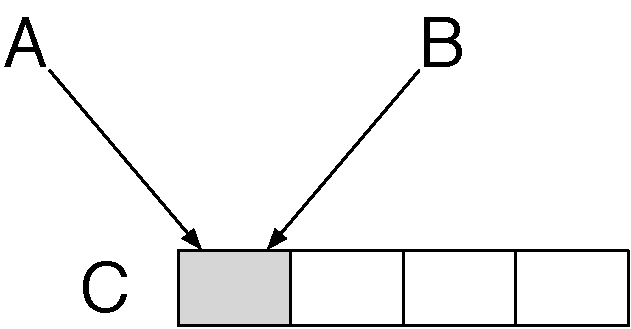
\includegraphics[width=0.5\textwidth]{graphics/aliasing.pdf}
		\caption{Aliasing example with A and B pointing to the same array C}
		\label{fig:aliasing}
	\end{figure}
	
	Although this may seem like an issue for lower-level programming languages, it can also exist in high(er) level languages such as Java:
	
	\begin{lstlisting}[caption=Aliasing in Java,caption=lst:javaalias]
		A[] a = new A[10];
		A[] b = a;\end{lstlisting}
	
	In some cases it may be useful to use such \textit{aliasing semantics}, for instance to reduce memory usage as pass-by-reference (or pointer passing) can be used instead of pass-by-value. Notice that doing so reduces further the `declarativeness' of the program - it gives the user more complete control over the specific layout of the data within memory.
	
	However, doing so creates implicit total ordering constraints on any operations using the aliased values. If these constraints are not matched -- \eg, if out-of-order or speculative execution is used -- the program correctness is no longer guaranteed. We can say that the two statements are dependent on each other, as described in section \ref{sec:runtime/analysis/theory}.
	
	Aliasing makes multi-threading more dangerous/difficult, and requires additional programmer effort. Firstly, if \texttt{A} and \texttt{B} are held by different threads (and note this scales for any $n > 1$ threads), then some kind of protection (such as locking or transactional memory) must be used in order to prevent inconsistencies resulting from concurrent access. The use of locking and synchronisation does however introduce a performance penalty. Note that even if synchronisation is used, the order of access must \emph{also} be controlled as otherwise the effect would be the same as it would for out-of-order or speculative execution -- non-deterministic results. Given this, we can conclude that multi-threading with aliased pointers/references implies single-threaded performance as access order and locking must be satisfied.

\section{Solutions} \label{sec:parametric/solutions}
There are several solutions that are possible, we consider several here.

	\subsection{Single-Command, Dual Value} \label{sec:parametric/solutions/scdv}

\section{Implementation Details} \label{sec:parametric/implementation}

\section{Additional Parameters} \label{sec:parametric/additional-params}

\section{Summary} \label{sec:parametric/summary}
In this section, a new kind of benchmark has been introduced. This benchmark is capable of producing configurations for various computations involving the three different dependency types (see section \ref{sec:runtime/analysis}). The problem statement for such a benchmark has been introduced, as well as possible solutions and implementation details of the chosen solution. Such a benchmark is likely useful to the wider parallelism community, so we included various additional parameters, such as the `amount of computation' done per cycle (which can be configured dynamically).